% Options for packages loaded elsewhere
\PassOptionsToPackage{unicode}{hyperref}
\PassOptionsToPackage{hyphens}{url}
\PassOptionsToPackage{dvipsnames,svgnames,x11names}{xcolor}
%
\documentclass[
  letterpaper,
  DIV=11,
  numbers=noendperiod]{scrartcl}

\usepackage{amsmath,amssymb}
\usepackage{iftex}
\ifPDFTeX
  \usepackage[T1]{fontenc}
  \usepackage[utf8]{inputenc}
  \usepackage{textcomp} % provide euro and other symbols
\else % if luatex or xetex
  \usepackage{unicode-math}
  \defaultfontfeatures{Scale=MatchLowercase}
  \defaultfontfeatures[\rmfamily]{Ligatures=TeX,Scale=1}
\fi
\usepackage{lmodern}
\ifPDFTeX\else  
    % xetex/luatex font selection
\fi
% Use upquote if available, for straight quotes in verbatim environments
\IfFileExists{upquote.sty}{\usepackage{upquote}}{}
\IfFileExists{microtype.sty}{% use microtype if available
  \usepackage[]{microtype}
  \UseMicrotypeSet[protrusion]{basicmath} % disable protrusion for tt fonts
}{}
\makeatletter
\@ifundefined{KOMAClassName}{% if non-KOMA class
  \IfFileExists{parskip.sty}{%
    \usepackage{parskip}
  }{% else
    \setlength{\parindent}{0pt}
    \setlength{\parskip}{6pt plus 2pt minus 1pt}}
}{% if KOMA class
  \KOMAoptions{parskip=half}}
\makeatother
\usepackage{xcolor}
\setlength{\emergencystretch}{3em} % prevent overfull lines
\setcounter{secnumdepth}{5}
% Make \paragraph and \subparagraph free-standing
\makeatletter
\ifx\paragraph\undefined\else
  \let\oldparagraph\paragraph
  \renewcommand{\paragraph}{
    \@ifstar
      \xxxParagraphStar
      \xxxParagraphNoStar
  }
  \newcommand{\xxxParagraphStar}[1]{\oldparagraph*{#1}\mbox{}}
  \newcommand{\xxxParagraphNoStar}[1]{\oldparagraph{#1}\mbox{}}
\fi
\ifx\subparagraph\undefined\else
  \let\oldsubparagraph\subparagraph
  \renewcommand{\subparagraph}{
    \@ifstar
      \xxxSubParagraphStar
      \xxxSubParagraphNoStar
  }
  \newcommand{\xxxSubParagraphStar}[1]{\oldsubparagraph*{#1}\mbox{}}
  \newcommand{\xxxSubParagraphNoStar}[1]{\oldsubparagraph{#1}\mbox{}}
\fi
\makeatother


\providecommand{\tightlist}{%
  \setlength{\itemsep}{0pt}\setlength{\parskip}{0pt}}\usepackage{longtable,booktabs,array}
\usepackage{calc} % for calculating minipage widths
% Correct order of tables after \paragraph or \subparagraph
\usepackage{etoolbox}
\makeatletter
\patchcmd\longtable{\par}{\if@noskipsec\mbox{}\fi\par}{}{}
\makeatother
% Allow footnotes in longtable head/foot
\IfFileExists{footnotehyper.sty}{\usepackage{footnotehyper}}{\usepackage{footnote}}
\makesavenoteenv{longtable}
\usepackage{graphicx}
\makeatletter
\def\maxwidth{\ifdim\Gin@nat@width>\linewidth\linewidth\else\Gin@nat@width\fi}
\def\maxheight{\ifdim\Gin@nat@height>\textheight\textheight\else\Gin@nat@height\fi}
\makeatother
% Scale images if necessary, so that they will not overflow the page
% margins by default, and it is still possible to overwrite the defaults
% using explicit options in \includegraphics[width, height, ...]{}
\setkeys{Gin}{width=\maxwidth,height=\maxheight,keepaspectratio}
% Set default figure placement to htbp
\makeatletter
\def\fps@figure{htbp}
\makeatother
% definitions for citeproc citations
\NewDocumentCommand\citeproctext{}{}
\NewDocumentCommand\citeproc{mm}{%
  \begingroup\def\citeproctext{#2}\cite{#1}\endgroup}
\makeatletter
 % allow citations to break across lines
 \let\@cite@ofmt\@firstofone
 % avoid brackets around text for \cite:
 \def\@biblabel#1{}
 \def\@cite#1#2{{#1\if@tempswa , #2\fi}}
\makeatother
\newlength{\cslhangindent}
\setlength{\cslhangindent}{1.5em}
\newlength{\csllabelwidth}
\setlength{\csllabelwidth}{3em}
\newenvironment{CSLReferences}[2] % #1 hanging-indent, #2 entry-spacing
 {\begin{list}{}{%
  \setlength{\itemindent}{0pt}
  \setlength{\leftmargin}{0pt}
  \setlength{\parsep}{0pt}
  % turn on hanging indent if param 1 is 1
  \ifodd #1
   \setlength{\leftmargin}{\cslhangindent}
   \setlength{\itemindent}{-1\cslhangindent}
  \fi
  % set entry spacing
  \setlength{\itemsep}{#2\baselineskip}}}
 {\end{list}}
\usepackage{calc}
\newcommand{\CSLBlock}[1]{\hfill\break\parbox[t]{\linewidth}{\strut\ignorespaces#1\strut}}
\newcommand{\CSLLeftMargin}[1]{\parbox[t]{\csllabelwidth}{\strut#1\strut}}
\newcommand{\CSLRightInline}[1]{\parbox[t]{\linewidth - \csllabelwidth}{\strut#1\strut}}
\newcommand{\CSLIndent}[1]{\hspace{\cslhangindent}#1}

\usepackage{booktabs}
\usepackage{longtable}
\usepackage{array}
\usepackage{multirow}
\usepackage{wrapfig}
\usepackage{float}
\usepackage{colortbl}
\usepackage{pdflscape}
\usepackage{tabu}
\usepackage{threeparttable}
\usepackage{threeparttablex}
\usepackage[normalem]{ulem}
\usepackage{makecell}
\usepackage{xcolor}
\KOMAoption{captions}{tableheading}
\makeatletter
\@ifpackageloaded{caption}{}{\usepackage{caption}}
\AtBeginDocument{%
\ifdefined\contentsname
  \renewcommand*\contentsname{Table of contents}
\else
  \newcommand\contentsname{Table of contents}
\fi
\ifdefined\listfigurename
  \renewcommand*\listfigurename{List of Figures}
\else
  \newcommand\listfigurename{List of Figures}
\fi
\ifdefined\listtablename
  \renewcommand*\listtablename{List of Tables}
\else
  \newcommand\listtablename{List of Tables}
\fi
\ifdefined\figurename
  \renewcommand*\figurename{Figure}
\else
  \newcommand\figurename{Figure}
\fi
\ifdefined\tablename
  \renewcommand*\tablename{Table}
\else
  \newcommand\tablename{Table}
\fi
}
\@ifpackageloaded{float}{}{\usepackage{float}}
\floatstyle{ruled}
\@ifundefined{c@chapter}{\newfloat{codelisting}{h}{lop}}{\newfloat{codelisting}{h}{lop}[chapter]}
\floatname{codelisting}{Listing}
\newcommand*\listoflistings{\listof{codelisting}{List of Listings}}
\makeatother
\makeatletter
\makeatother
\makeatletter
\@ifpackageloaded{caption}{}{\usepackage{caption}}
\@ifpackageloaded{subcaption}{}{\usepackage{subcaption}}
\makeatother

\ifLuaTeX
  \usepackage{selnolig}  % disable illegal ligatures
\fi
\usepackage{bookmark}

\IfFileExists{xurl.sty}{\usepackage{xurl}}{} % add URL line breaks if available
\urlstyle{same} % disable monospaced font for URLs
\hypersetup{
  pdftitle={Forecasting Stock Market Dynamics in the Tech Sector: A Multi-Stock Gradient Boosting Approach},
  pdfauthor={Jamie Lee},
  colorlinks=true,
  linkcolor={blue},
  filecolor={Maroon},
  citecolor={Blue},
  urlcolor={Blue},
  pdfcreator={LaTeX via pandoc}}


\title{Forecasting Stock Market Dynamics in the Tech Sector: A
Multi-Stock Gradient Boosting Approach\thanks{Code and data are
available at: https://github.com/jamiejiminlee/Tech-Stock-Forecast.git}}
\author{Jamie Lee}
\date{November 21, 2024}

\begin{document}
\maketitle
\begin{abstract}
First sentence. Second sentence. Third sentence. Fourth sentence.
\end{abstract}


\section{Introduction}\label{introduction}

Overview paragraph

Estimand paragraph

Results paragraph

Why it matters paragraph

Telegraphing paragraph: The remainder of this paper is structured as
follows. Section~\ref{sec-data}\ldots.

\section{Data}\label{sec-data}

\subsection{Overview}\label{overview}

The data for this paper, obtained from the Yahoo Finance API via the
\texttt{tidyquant} by library in R on November 19, 2024, encompasses
historical stock price information for four leading technology
companies: Google (GOOG), Apple (AAPL), Amazon (AMZN), and Microsoft
(MSFT). This dataset spans from January 1, 2018, to December 31, 2024,
providing daily stock market data for each company. Key variables
include \textbf{\texttt{symbol}}, \textbf{\texttt{date}},
\textbf{\texttt{open}}, \textbf{\texttt{high}}, \textbf{\texttt{low}},
\textbf{\texttt{close}}, \textbf{\texttt{volume}}, and
\textbf{\texttt{adjusted}} prices. Our analysis focuses on predicting
daily price differences and percentage changes across this basket of
stocks, leveraging additional features constructed from the raw dataset.
These features include \textbf{\texttt{Price\_Lag1}} (lagged closing
prices), \textbf{\texttt{Price\_Diff}} (daily price differences), and
\textbf{\texttt{Price\_Change\_Percent}} (percentage changes). By
incorporating these derived variables, we aim to capture sequential
trends and normalize differences across stocks with varying price
ranges.

To ensure reliability, the data was pre-processed to remove missing
values, align time-frames across stocks, and compute the constructed
variables. Observations with incomplete data were excluded to maintain
consistency in analysis. Data cleaning and analysis were conducted using
the following packages: the \texttt{tidyverse} package of
(\textbf{Tidyverse?}), \texttt{lubridate} package of
(\textbf{Lubridate?}), and \texttt{arrow} package of (\textbf{arrow?}).
Details on the data cleaning and manipulation process are provided in
\textbf{?@sec-data-cleaning}.

\subsection{Measurement}\label{measurement}

Stock prices are influenced by numerous factors, including macroeconomic
conditions, industry trends, corporate actions, and investor sentiment.
These dynamics fluctuate frequently, often in response to earnings
reports, geopolitical events, or shifts in market expectations.
Financial data simplifies these complex market behaviors into numerical
indicators such as \textbf{\texttt{open}}, \textbf{\texttt{high}},
\textbf{\texttt{low}}, and \textbf{\texttt{close}} prices, which, while
precise, may not fully encapsulate underlying investor motivations or
market sentiment. For instance, the closing price represents only the
last traded price of the day, smoothing out intraday volatility and
obscuring more nuanced trading patterns.

Constructed variables like \textbf{\texttt{Price\_Diff}} and
\textbf{\texttt{Price\_Change\_Percent}} aim to quantify daily stock
price movements by measuring differences or proportional changes
relative to the previous day. However, these metrics assume that price
movements reflect consistent investor sentiment across all stocks,
potentially overlooking idiosyncratic factors specific to individual
companies, such as leadership changes or product launches. Additionally,
these metrics equally weight all days, despite certain trading days
(e.g., earnings announcements or market holidays) being more
influential.

The \textbf{\texttt{volume}} variable, representing the total shares
traded, is used as a proxy for market activity and investor interest.
This assumes that higher trading volumes uniformly indicate significant
market events, despite possible differences in trading motives, such as
speculative activity or algorithmic trading. Similarly, the temporal
predictors, including \textbf{\texttt{date}},
\textbf{\texttt{day\ of\ the\ week}}, and \textbf{\texttt{month}}, aim
to capture seasonal trends or trading patterns. However, these features
simplify complex market behaviors into discrete time intervals,
potentially overlooking shorter-term dynamics like market reactions to
breaking news or macroeconomic data releases.

By aggregating these variables across a basket of stocks, the model
assumes comparability among them, despite differences in market
capitalization, industry focus, and investor bases. This simplification
may obscure unique drivers of price changes for each stock, potentially
limiting the model's ability to capture more granular patterns.
Nonetheless, these variables collectively provide a structured framework
for analyzing and predicting daily price movements within the selected
basket of stocks.

\subsection{Variables}\label{variables}

The collected data from Yahoo Finance includes several key variables
relevant to the analysis of price changes across a basket of tech stocks
(\textbf{Google}, \textbf{Apple}, \textbf{Amazon}, and
\textbf{Microsoft}). The original dataset contains the following
columns:

\begin{itemize}
\tightlist
\item
  \textbf{\texttt{symbol}}: Represents the stock ticker symbol,
  identifying the company (e.g., GOOG for Google, AAPL for Apple).
\item
  \textbf{\texttt{date}}: The trading date, essential for tracking and
  analyzing temporal patterns.
\item
  \textbf{\texttt{open}}: The stock's opening price on a given day,
  providing context for daily price movements.
\item
  \textbf{\texttt{high}}: The highest price of the stock during the
  trading day, useful for understanding intraday volatility.
\item
  \textbf{\texttt{low}}: The lowest price of the stock during the
  trading day, another measure of volatility.
\item
  \textbf{\texttt{close}}: The stock's closing price on a given day,
  which is a standard benchmark for daily performance.
\item
  \textbf{\texttt{volume}}: The total number of shares traded during the
  day, reflecting market activity and investor interest.
\item
  \textbf{\texttt{adjusted}}: The adjusted closing price, accounting for
  corporate actions like stock splits and dividends to provide a
  standardized measure of value.
\end{itemize}

In addition to these original variables, new features were constructed
to enhance the analysis:

\begin{itemize}
\tightlist
\item
  \textbf{\texttt{Price\_Lag1}}: Derived as the closing price from the
  previous trading day, enabling the analysis of sequential price
  changes.
\item
  \textbf{\texttt{Price\_Diff}}: Calculated as the difference between
  the current day's closing price and the previous day's closing price,
  capturing day-to-day fluctuations.
\item
  \textbf{\texttt{Price\_Change\_Percent}}: Derived as the percentage
  change in stock price relative to the previous day's closing price,
  normalized to enable comparisons across stocks.
\end{itemize}

These constructed variables allow for a more detailed examination of
stock price movements. To ensure high-quality analysis, the data was
cleaned and preprocessed to remove missing values, align timeframes
across stocks, and compute these derived features. For further details
on the data cleaning and preparation process, refer to
\textbf{?@sec-data-cleaning}.

\subsubsection{Outcome Variables}\label{outcome-variables}

The outcome variable for this paper is the \textbf{Daily Percentage
Change (\texttt{Price\_Change\_Percent})}, which measures the
proportional change in a stock's closing price relative to its previous
day's closing price. This variable is calculated as:

\[
\text{Price_Change_Percent} = \frac{\text{close} - \text{Price_Lag1}}{\text{Price_Lag1}} \times 100
\] This metric normalizes price movements across the basket of stocks,
enabling meaningful comparisons despite differences in price ranges
between stocks such as Google (\textbf{GOOG}), Apple (\textbf{AAPL}),
Amazon (\textbf{AMZN}), and Microsoft (\textbf{MSFT}). By focusing on
percentage changes, the analysis captures the relative daily performance
of each stock, providing insights into trends and volatility. This
variable is widely used in financial analysis to track and compare stock
performance over time, making it a suitable choice for this study.

\begin{figure}

\centering{

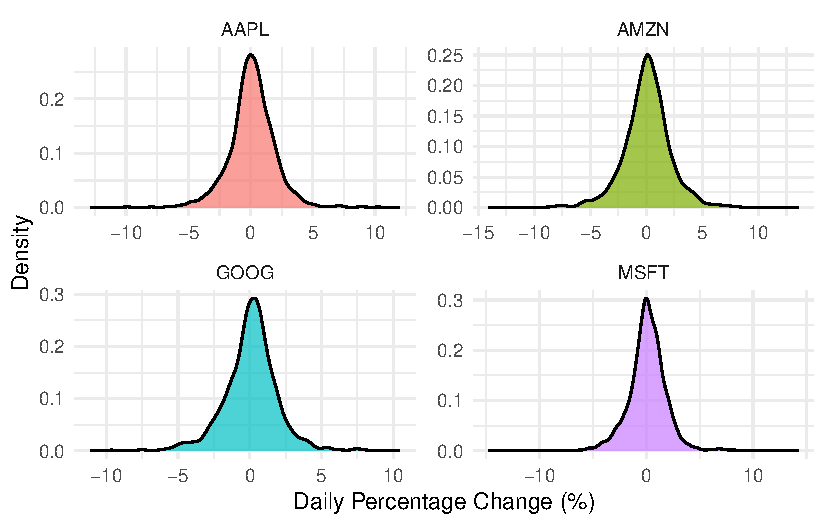
\includegraphics{paper_files/figure-pdf/fig-outcome-var-1.pdf}

}

\caption{\label{fig-outcome-var}Distribution of Daily Percentage Changes
by Stock}

\end{figure}%

Figure~\ref{fig-outcome-var} above illustrates the distribution of
\textbf{Daily Percentage Changes (\texttt{Price\_Change\_Percent})} for
each stock in the basket: Apple (\textbf{AAPL}), Amazon (\textbf{AMZN}),
Google (\textbf{GOOG}), and Microsoft (\textbf{MSFT}). Each panel
represents a stock, providing a separate density curve that highlights
its unique distribution pattern. Across all stocks, the distributions
exhibit a sharp central peak around 0\%, indicating that most daily
percentage changes are minor. However, the tails of the distributions
reveal occasional larger price movements, both positive and negative,
reflecting the volatility inherent in stock markets. Notably, the widths
of the distributions differ slightly among the stocks, with Amazon
(AMZN) displaying a broader tail, suggesting higher variability in its
daily percentage changes compared to others.

\subsubsection{Predictor variables}\label{predictor-variables}

To forecast the daily percentage changes in stock prices
(\textbf{\texttt{Price\_Change\_Percent}}), several predictor variables
are utilized, derived from the cleaned dataset. These predictors
encompass historical price trends, market activity metrics, and temporal
features, offering a comprehensive framework for modeling stock price
behavior:

\begin{itemize}
\item
  \textbf{\texttt{Price\_Lag1}}: The closing price of the stock on the
  previous trading day. This variable captures the most recent
  historical price trend, which is often a strong predictor of
  subsequent price movements.
\item
  \textbf{\texttt{volume}}: The total number of shares traded on a given
  day. This variable reflects market activity and investor interest,
  with higher volumes often indicating significant events or changes in
  sentiment.
\item
  \textbf{\texttt{open}}: The stock's opening price on a given day. This
  metric provides context for intraday price dynamics and can indicate
  whether the day begins with positive or negative momentum.
\item
  \textbf{\texttt{high}}: The highest price the stock reached during the
  trading day. This variable highlights the potential upward volatility
  within the day, offering insights into optimistic trading behavior.
\item
  \textbf{\texttt{low}}: The lowest price the stock reached during the
  trading day. This variable captures the potential downward volatility,
  reflecting pessimistic market behavior.
\item
  \textbf{\texttt{adjusted}}: The adjusted closing price, which accounts
  for corporate actions like stock splits and dividends. This ensures a
  standardized measure of value over time, enabling better comparisons
  across stocks.
\item
  \textbf{\texttt{date}}: The trading date, used to derive temporal
  features such as the day of the week and the month. Temporal variables
  capture seasonal trends and trading patterns that can influence stock
  prices.
\end{itemize}

These predictor variables enables the model to incorporate historical
price trends, market dynamics, and seasonal influences, providing a
robust basis for forecasting daily percentage changes in stock prices.
By leveraging this diverse set of predictors, the analysis aims to
identify patterns and relationships that drive stock price fluctuations
across the basket of tech stocks.

\begin{longtable}[]{@{}
  >{\raggedright\arraybackslash}p{(\columnwidth - 14\tabcolsep) * \real{0.1102}}
  >{\raggedright\arraybackslash}p{(\columnwidth - 14\tabcolsep) * \real{0.0932}}
  >{\raggedleft\arraybackslash}p{(\columnwidth - 14\tabcolsep) * \real{0.2373}}
  >{\raggedleft\arraybackslash}p{(\columnwidth - 14\tabcolsep) * \real{0.0847}}
  >{\raggedleft\arraybackslash}p{(\columnwidth - 14\tabcolsep) * \real{0.1186}}
  >{\raggedleft\arraybackslash}p{(\columnwidth - 14\tabcolsep) * \real{0.1186}}
  >{\raggedleft\arraybackslash}p{(\columnwidth - 14\tabcolsep) * \real{0.1102}}
  >{\raggedleft\arraybackslash}p{(\columnwidth - 14\tabcolsep) * \real{0.1271}}@{}}

\caption{\label{tbl-pred-var}Sample of Predictor Variables}

\tabularnewline

\toprule\noalign{}
\begin{minipage}[b]{\linewidth}\raggedright
Stock Symbol
\end{minipage} & \begin{minipage}[b]{\linewidth}\raggedright
Date
\end{minipage} & \begin{minipage}[b]{\linewidth}\raggedleft
Previous Close (Price\_Lag1)
\end{minipage} & \begin{minipage}[b]{\linewidth}\raggedleft
Volume
\end{minipage} & \begin{minipage}[b]{\linewidth}\raggedleft
Opening Price
\end{minipage} & \begin{minipage}[b]{\linewidth}\raggedleft
Highest Price
\end{minipage} & \begin{minipage}[b]{\linewidth}\raggedleft
Lowest Price
\end{minipage} & \begin{minipage}[b]{\linewidth}\raggedleft
Adjusted Close
\end{minipage} \\
\midrule\noalign{}
\endhead
\bottomrule\noalign{}
\endlastfoot
GOOG & 2021-10-18 & 141.68 & 16564000 & 141.21 & 143.00 & 141.21 &
142.61 \\
AAPL & 2018-09-20 & 54.59 & 106435200 & 55.06 & 55.57 & 54.79 & 52.36 \\
MSFT & 2024-01-23 & 396.51 & 20525900 & 395.75 & 399.38 & 393.93 &
396.73 \\
MSFT & 2023-11-03 & 348.32 & 23624000 & 349.63 & 354.39 & 347.33 &
350.17 \\
GOOG & 2021-08-02 & 135.22 & 20140000 & 135.48 & 136.02 & 134.67 &
135.66 \\

\end{longtable}

Table~\ref{tbl-pred-var} displays a random sample of five rows from the
dataset, showcasing the predictor variables used in the analysis. These
variables include \textbf{stock symbol}, \textbf{date}, \textbf{previous
day's closing price (\(\text{Price\_Lag1}\))}, \textbf{volume},
\textbf{opening price}, \textbf{highest price}, \textbf{lowest price},
and \textbf{adjusted closing price}. The data highlights the variability
across stocks and trading days, with differences in prices and trading
volumes reflecting unique market conditions. For instance, Google (GOOG)
on 2024-07-18 had a closing price of \$182.62, while Apple (AAPL) on
2023-03-13 exhibited significant movement, with a high of \$153.14 and a
low of \$147.70. These variables collectively provide a robust
foundation for modeling and forecasting daily percentage changes in
stock prices.

\section{Model}\label{model}

\subsection{Model Overview}\label{model-overview}

This analysis employs an \textbf{XGBoost (R Core Team 2023) regression
model} to predict daily stock price changes, specifically focusing on
the variable Price\_Diff, which measures the difference in stock prices
from one trading day to the next. By leveraging key predictors derived
from historical data and stock market activity, the model identifies
patterns and trends that inform short-term price movements. The XGBoost
algorithm was selected for its efficiency and ability to handle large
datasets, as well as its effectiveness in capturing non-linear
relationships and interactions among variables. Background details and
diagnostics are included in Appendix~\ref{sec-model-details}.

\subsection{Model Assumptions}\label{model-assumptions}

The XGBoost regression model used in this analysis relies on several key
assumptions:

\begin{itemize}
\item
  \textbf{Independence of Observations}: The daily percentage changes in
  stock prices are assumed to be independent of each other. This implies
  that the prediction for one day does not influence or depend on the
  prediction for other days.
\item
  \textbf{Relevance of Predictors}: The chosen predictors (e.g.,
  \texttt{Price\_Lag1}, \texttt{Price\_Change\_Percent},
  \texttt{volume}, \texttt{open}, \texttt{high}, \texttt{low}, and
  \texttt{adjusted}) are assumed to adequately capture the key factors
  driving stock price changes. The model assumes no critical predictive
  variable is missing.
\item
  \textbf{Stationarity of Features}: The statistical properties of the
  predictors, such as their mean and variance, are assumed to remain
  stable over time within the training and testing periods. This is
  crucial for the model to generalize well to future data.
\item
  \textbf{No Multicollinearity}: The predictors are assumed to not be
  highly correlated with each other. Although gradient boosting models
  are robust to some multicollinearity, extreme collinearity could still
  negatively affect feature importance and model interpretation.
\item
  \textbf{Consistency of Temporal Effects}: Temporal variables, such as
  \texttt{date} and derived features like day of the week, are assumed
  to capture stable patterns in stock price movements across the
  training and testing periods.
\item
  \textbf{Additivity of Effects}: The model assumes that the combined
  effects of the predictors on the outcome variable
  (\texttt{Price\_Diff}) can be captured additively through the boosting
  algorithm. Non-linear interactions are handled automatically by
  XGBoost, but this assumption helps guide the model design.
\item
  \textbf{Complete Data}: The model assumes that missing data has been
  appropriately handled during preprocessing. This includes imputation,
  removal, or encoding of missing values.
\end{itemize}

These assumptions form the foundation of the modeling approach.
Addressing potential violations, such as temporal dependencies or
changes in feature distributions, will be discussed in the limitations
section.

\subsection{Model Setup}\label{model-setup}

Define \(y_i\) as the daily price difference for a given stock on day
\(i\). The predictors include \(\text{Price\_Lag1}_i\), the lagged
closing price, and other market and temporal features such as
\(\text{volume}_i\), \(\text{open}_i\), \(\text{high}_i\),
\(\text{low}_i\), and \(\text{adjusted}_i\). The relationship is modeled
as:

\[
y_i = f(X_i) + \epsilon_i
\]

where \(X_i\) is the set of predictors for observation \(i\), \(f(X_i)\)
is the function learned by the XGBoost model, and \(\epsilon_i\)
represents the residual error.

The model parameters are optimized to minimize the following objective
function:

\[
\mathcal{L}(\Theta) = \sum_{i=1}^N \left(y_i - f(X_i)\right)^2 + \Omega(f)
\]

where \(\mathcal{L}(\Theta)\) is the loss function, \(\Theta\)
represents the model parameters, and \(\Omega(f)\) is a regularization
term to prevent overfitting.

The model is implemented using the \texttt{xgboost} package in R. The
training dataset includes observations up to December 31, 2024, while
the testing dataset covers January to March 2025. The predictors
(\(X_i\)) used include:

\begin{itemize}
\tightlist
\item
  \(\text{Price\_Lag1}\): Previous day's closing price,
\item
  \(\text{Price\_Change\_Percent}\): Percentage change from the previous
  day,
\item
  \(\text{volume}\): Number of shares traded,
\item
  \(\text{open, high, low, adjusted}\): Daily stock metrics.
\end{itemize}

Key hyperparameters for the model are:

\begin{itemize}
\tightlist
\item
  Learning rate (\(\eta\)): \(0.1\)
\item
  Maximum tree depth: \(6\)
\item
  Number of boosting rounds: \(100\)
\item
  Sub Sample ratio: \(0.8\)
\item
  Column sampling ratio: \(0.8\)
\end{itemize}

These hyperparameters are tuned to balance predictive accuracy and
prevent overfitting, allowing the model to capture complex relationships
in stock price dynamics effectively. Details are further described in
Section~\ref{sec-model-summary}.

\subsection{Model justification}\label{model-justification}

The XGBoost regression model is the most suitable approach for
predicting daily price differences (\textbf{`Price\_Diff'}) across a
basket of tech stocks, including Google (\textbf{GOOG}), Apple
(\textbf{AAPL}), Amazon (\textbf{AMZN}), and Microsoft (\textbf{MSFT}).
By employing gradient boosting to iteratively minimize prediction
errors, XGBoost effectively handles the complex, non-linear
relationships inherent in stock price movements. It is particularly
well-suited for continuous outcomes like \textbf{`Price\_Diff'}, which
exhibit significant variability driven by historical trends, market
activity, and temporal effects. The model's ability to optimize squared
error loss while incorporating regularization prevents overfitting and
enhances generalizability. Additionally, XGBoost is robust to missing
data, automatically manages variable interactions, and is
computationally efficient, making it ideal for large datasets in
financial analysis.

While alternative approaches, such as traditional linear regression
models, could be used, they may not capture the complex interactions
between predictors like \texttt{Price\_Lag1},
\textbf{\texttt{Price\_Change\_Percent}}, and \textbf{\texttt{volume}}.
Machine learning models like random forests or neural networks offer
high flexibility but may sacrifice computational efficiency and
interpretability compared to XGBoost.

\subsection{Model Summary}\label{sec-model-summary}

The model's hyperparameters, set to optimize predictive accuracy and
computational efficiency, are displayed in \textbf{?@tbl-model} results.
It reveals 100 boosting rounds with a learning rate (\(\eta\)) of 0.1,
balancing fast convergence and overfitting control. A maximum tree depth
of 6 captures complex interactions among predictors without overfitting.
Column and row sampling rates of 0.8 each ensure robustness by
introducing randomness into feature and observation selection during
tree construction.

\begin{longtable}[t]{ll}

\caption{\label{tbl-modelsummary}Summary of XGBoost Model
Hyperparameters}

\tabularnewline

\toprule
Parameter & Value\\
\midrule
Number of Trees (Rounds) & 100\\
Learning Rate (eta) & 0.1\\
Max Tree Depth & 6\\
Column Sampling Rate & 0.8\\
Row Sampling Rate & 0.8\\
\addlinespace
Objective Function & Squared Error Regression (reg:squarederror)\\
\bottomrule

\end{longtable}

Furthermore, the model employs the squared error regression objective
function (\texttt{reg:squarederror}), suitable for continuous outcome
variables like \textbf{\texttt{Price\_Diff}}. These hyperparameters
enable the model to handle the non-linear relationships and variability
inherent in financial data effectively.

\section{Results}\label{results}

Our results are summarized in \textbf{?@tbl-modelresults}.

\begin{figure}

\centering{

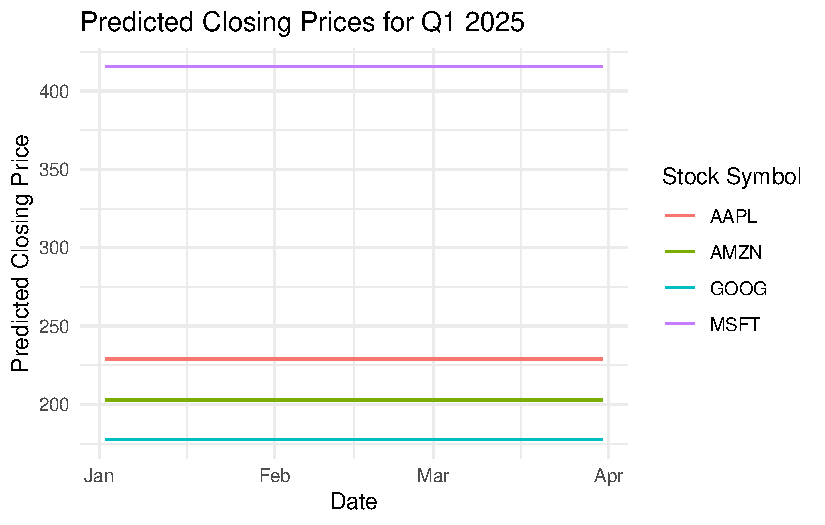
\includegraphics{paper_files/figure-pdf/fig-pred-price-1.pdf}

}

\caption{\label{fig-pred-price}Actual vs.~Predicted Daily Price
Differences}

\end{figure}%

\section{Discussion}\label{discussion}

\subsection{First discussion point}\label{sec-first-point}

If my paper were 10 pages, then should be be at least 2.5 pages. The
discussion is a chance to show off what you know and what you learnt
from all this.

\subsection{Second discussion point}\label{second-discussion-point}

Please don't use these as sub-heading labels - change them to be what
your point actually is.

\subsection{Third discussion point}\label{third-discussion-point}

\subsection{Weaknesses and next steps}\label{weaknesses-and-next-steps}

Weaknesses and next steps should also be included.

\newpage

\appendix

\section*{Appendix}\label{appendix}
\addcontentsline{toc}{section}{Appendix}

\section{Additional data details}\label{additional-data-details}

\section{Model details}\label{sec-model-details}

\subsection{Posterior predictive
check}\label{posterior-predictive-check}

In \textbf{?@fig-ppcheckandposteriorvsprior-1} we implement a posterior
predictive check. This shows\ldots{}

In \textbf{?@fig-ppcheckandposteriorvsprior-2} we compare the posterior
with the prior. This shows\ldots{}

\subsection{Diagnostics}\label{diagnostics}

\newpage

\section*{References}\label{references}
\addcontentsline{toc}{section}{References}

\phantomsection\label{refs}
\begin{CSLReferences}{1}{0}
\bibitem[\citeproctext]{ref-xgboost}
R Core Team. 2023. \emph{{R: A Language and Environment for Statistical
Computing}}. Vienna, Austria: R Foundation for Statistical Computing.
\url{https://www.R-project.org/}.

\end{CSLReferences}




\end{document}
